\documentclass[journal]{IEEEtran}
\usepackage[a5paper, margin=10mm, onecolumn]{geometry}
\usepackage[cmex10]{amsmath}
\usepackage{amssymb,amsfonts,amsthm}
\usepackage{gvv-book}
\usepackage{gvv}
\usepackage{hyperref}


\begin{document}
\title{8.4.28}
\author{EE25BTECH11025 - Ganachari Vishwambhar}
\maketitle

\textbf{Question}:\\
The axis of the parabola is along the line $y=x$ and trhe distance of its vertex and focus from origin are $\sqrt{2}$ and $2\sqrt{2}$ respectively. If the vertex and focus both lie in the first quadrant, then the equation of the parabola is
\begin{enumerate}
\begin{multicols}{2}
    \item $(x+y)^2=(x-y-2)$
    \item $(x-y)^2=(x+y-2)$
    \item $(x-y)^2=4(x+y-2)$
    \item $(x-y)^2=8(x+y-2)$
\end{multicols}
\end{enumerate}
\textbf{Solution: }\\
Let:\\
Focus of the parabola be $\vec{F}$\\
Vertex of the parabola be $\vec{V}$\\
Normal vector to the directrix be $\vec{n}$\\
The point of intersection of directrix and axis be $\vec{P}$\\
Direction vector and slope of axis be $\vec{m}_1$ and $m_1$\\
Direction vector and slope of directrix be $\vec{m}_2$ and $m_2$\\
Equation of axis be $\vec{x}=\lambda\vec{m}_1$\\
Given:
\begin{align}
    \norm{\vec{F}} = 2\sqrt{2}\\
    \norm{\vec{V}} = \sqrt{2}\\
    \vec{m}_1 = \myvec{1\\m_1}=\myvec{1\\1}
\end{align}

Finding focus($\vec{F}$):
\begin{align}
    \lambda\vec{m}_1=\vec{F}\\
    \lambda = \pm\frac{\norm{\vec{F}}}{\norm{\vec{m}_1}}\\
    \vec{F} = \pm\frac{\norm{\vec{F}}}{\norm{\vec{m}_1}}\vec{m}_1
\end{align}

Finding vertex($\vec{V}$)
\begin{align}
    \lambda\vec{m}_1=\vec{V}\\
    \lambda = \pm\frac{\norm{\vec{V}}}{\norm{\vec{m}_1}}\\
    \vec{V} = \pm\frac{\norm{\vec{V}}}{\norm{\vec{m}_1}}\vec{m}_1
\end{align}

Since directrix will be perpendicular to axis $m_1m_2=-1$
\begin{align}
    \vec{m_2} = \myvec{1\\m_2} = \myvec{1\\ \frac{-1}{m_1}}\\
    \vec{n} = \myvec{0&1\\-1&0}\vec{m_2}
\end{align}

Since $\vec{V}$ will be midpoint of $\vec{P}$ and $\vec{F}$ and also $\vec{P}$:
\begin{align}
    \frac{\vec{P}+\vec{F}}{2} = \vec{V}\\
    \vec{P}=2\vec{V}-\vec{F}
\end{align}

Now, finding the directrix equation in normal form;
\begin{align}
    \vec{n}^\top\vec{x}=\vec{n}^\top\vec{P}
\end{align}

From equation of conic $\vec{x}^\top A\vec{x}+2\vec{u}^\top\vec{x}+f=0$\\
For parabola:
\begin{align}
    A=\norm{\vec{n}}^2I-\vec{n}\vec{n}^\top\\
    \vec{u}=c\vec{n}-\norm{\vec{n}}^2\vec{F}=\vec{n}^2\vec{P}\vec{n}-\norm{\vec{n}}^2\frac{\norm{\vec{F}}}{\norm{\vec{m}_1}}\vec{m}_1\\
    f=\norm{\vec{n}}^2\norm{\vec{F}}^2-c^2=\norm{\vec{n}}^2\norm{\vec{F}}^2-\brak{\vec{n}^\top\vec{P}}^2
\end{align}

Substituting values given in question we get:
\begin{align}
    A=\myvec{1&-1\\-1&1}\\
    \vec{u}=-4\myvec{1\\1}\\
    f=16
\end{align}

Substituting (18), (19) and (20) in conic equation we get:
\begin{align}
    \myvec{x&y}\myvec{1&-1\\-1&1}\myvec{x\\y}+\brak{-4}\myvec{1&1}\myvec{x\\y}+16=0\\
    \brak{x+y}^2=8\brak{x+y-2}
\end{align}
Hnece, option(4) is correct.

\begin{figure}[h!]
   \centering
   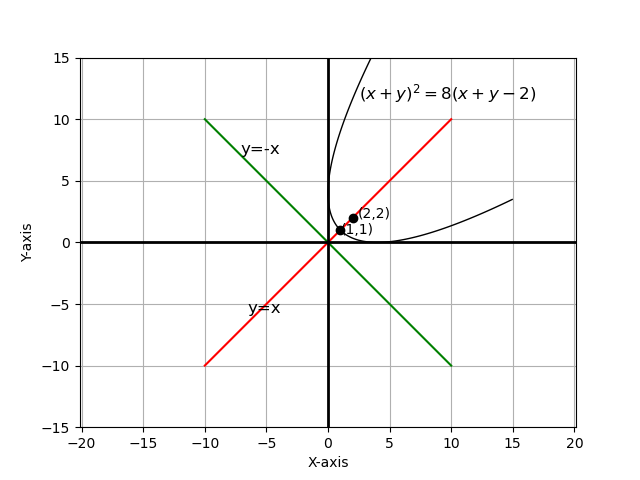
\includegraphics[width=0.7\linewidth]{figs/plot.png}
   \caption{Plot of the parabola}
   \label{}
\end{figure}

\end{document}
